\section{SNet - Freies Netz in Kuba}
\subsection{Why not diy?}

\begin{frame}
\frametitle{Staatliches Internet \& seine Flaws}
	\begin{itemize}
		\item Langsames \& teures Netz:
		\item Nur 1 Glasfaserleitung vom Festland
		\item Zugang kontrolliert von staatl. Telefongesellschaften
		\item WiFi-Hotspots verbreiteter als Festnetz
		\item Kosten bei ca. 1 Dollar / h. surfen
	\end{itemize}
\end{frame}

\subsection{SNet - Entstehung \& Verbreitung}

\begin{frame}
\frametitle{SNet - Entstehung \& Verbreitung}
	\begin{itemize}
		\item Die SNet-Community baut ihr eigenes Internet - nicht mit dem globalen Internet verbunden
		\item Entstand 2011 als Verknüpfung von Heimnetzwerken für Gaming \& Filesharing
		\item Mittlerweile Netzwerk aus mehr als 100.000 aktiven Nutzern
		\item Verteilung über Havanna:
			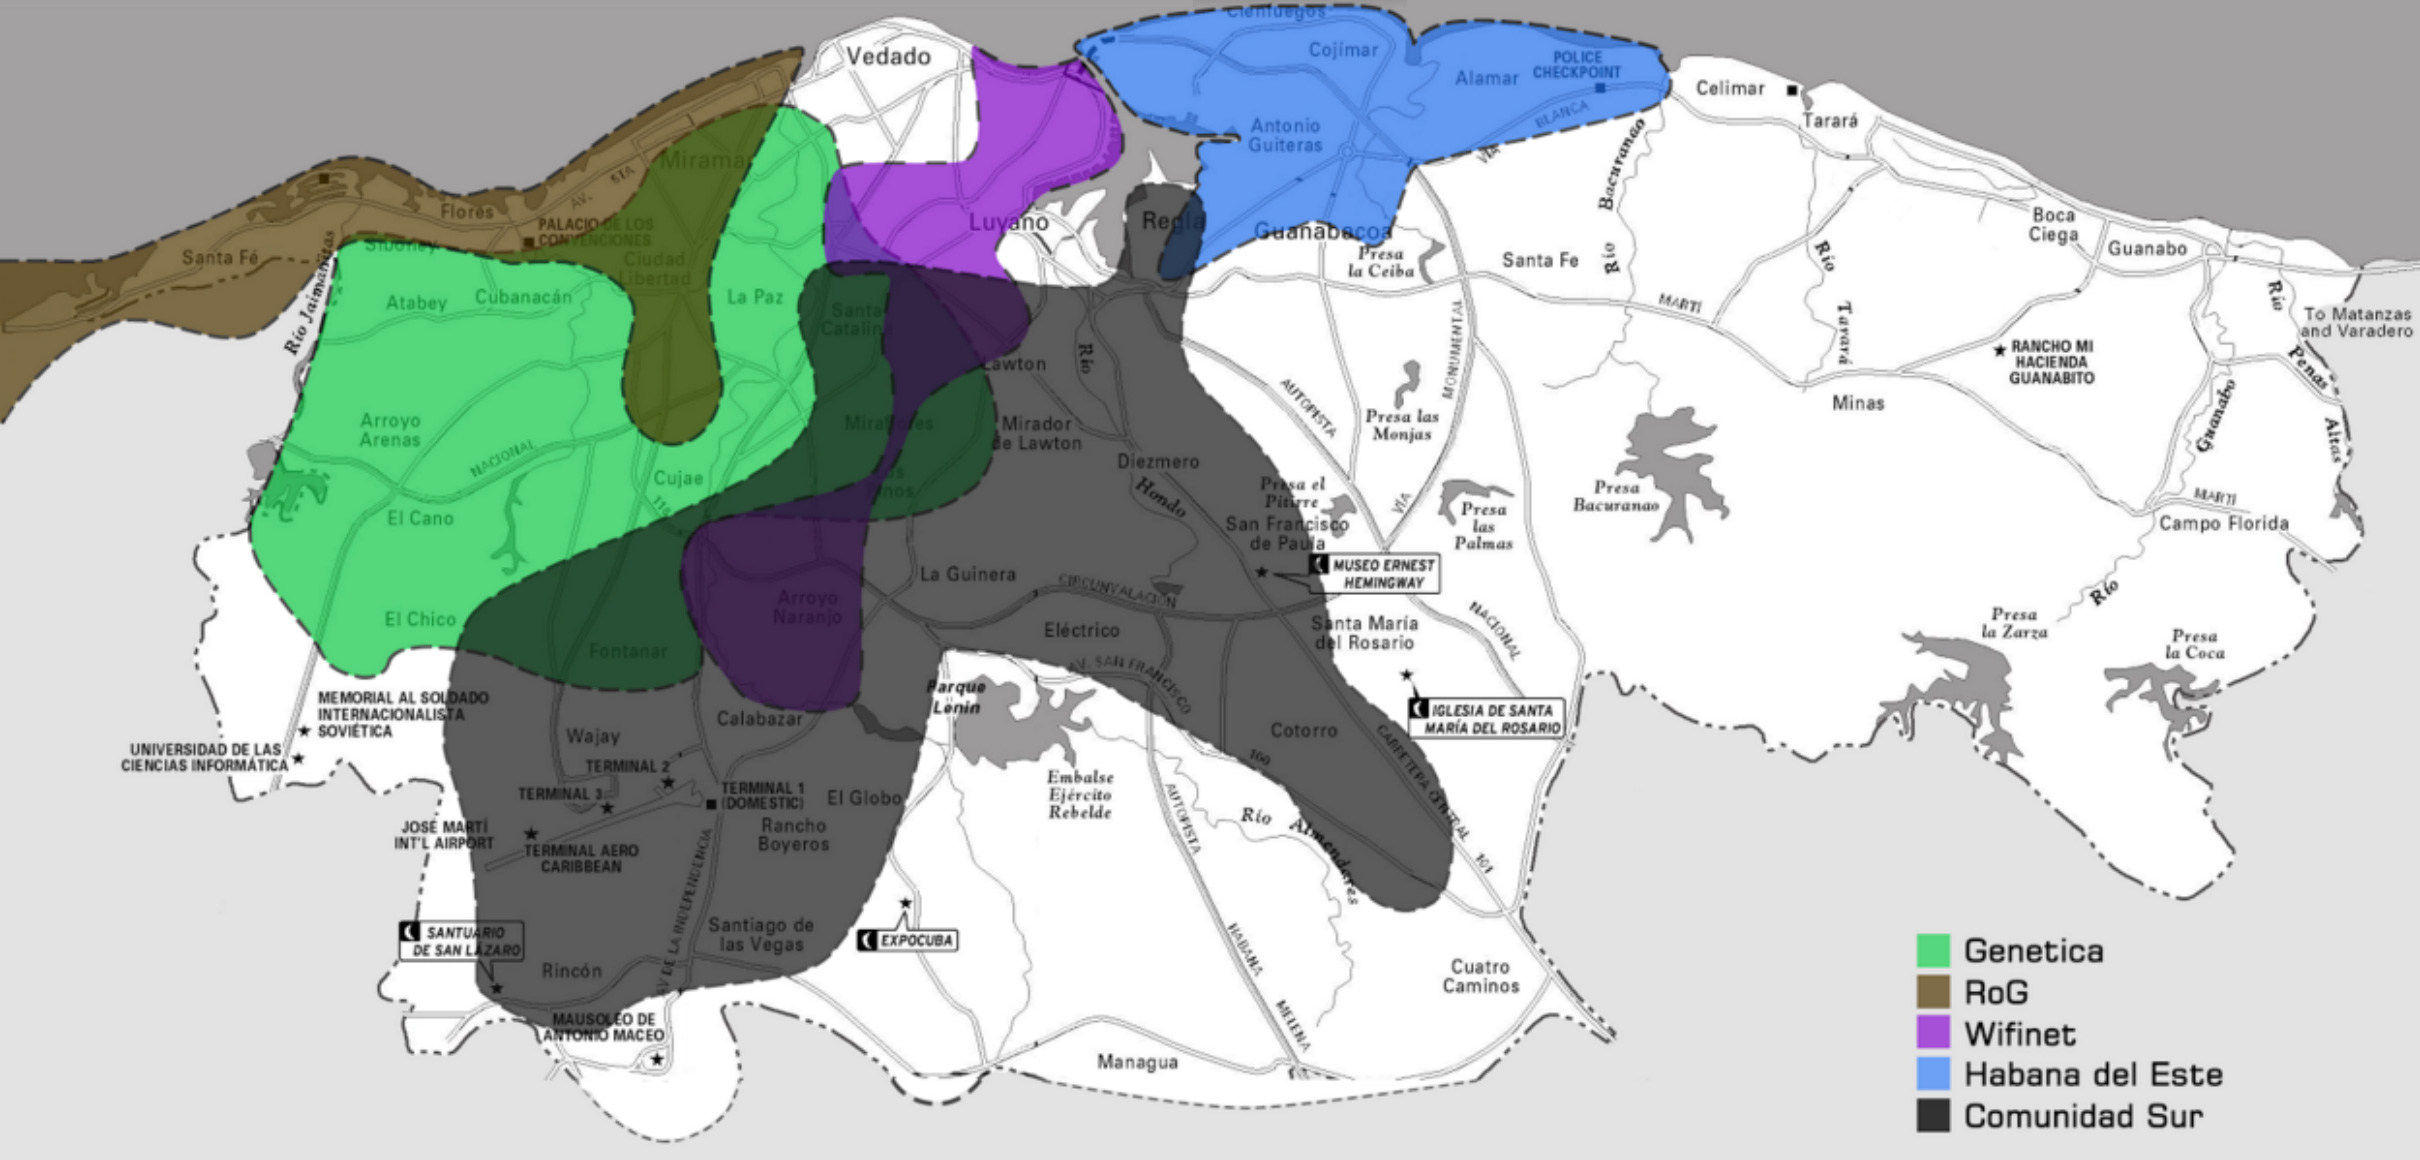
\includegraphics[width=\textwidth]{images/havanna_net.jpg}
	\end{itemize}
	
\end{frame}

\subsection{Technik, Hardware \& Autonomie}

\begin{frame}
\frametitle{Netz ohne Kontrolle von außen}
	\begin{itemize}
		\item SNet kommt ohne Verbindung zum globalen Internet aus
		\item Entgeht damit staatlichen Kontrollmechanismen
		\item Ist technisch recht leicht umsetzbar
			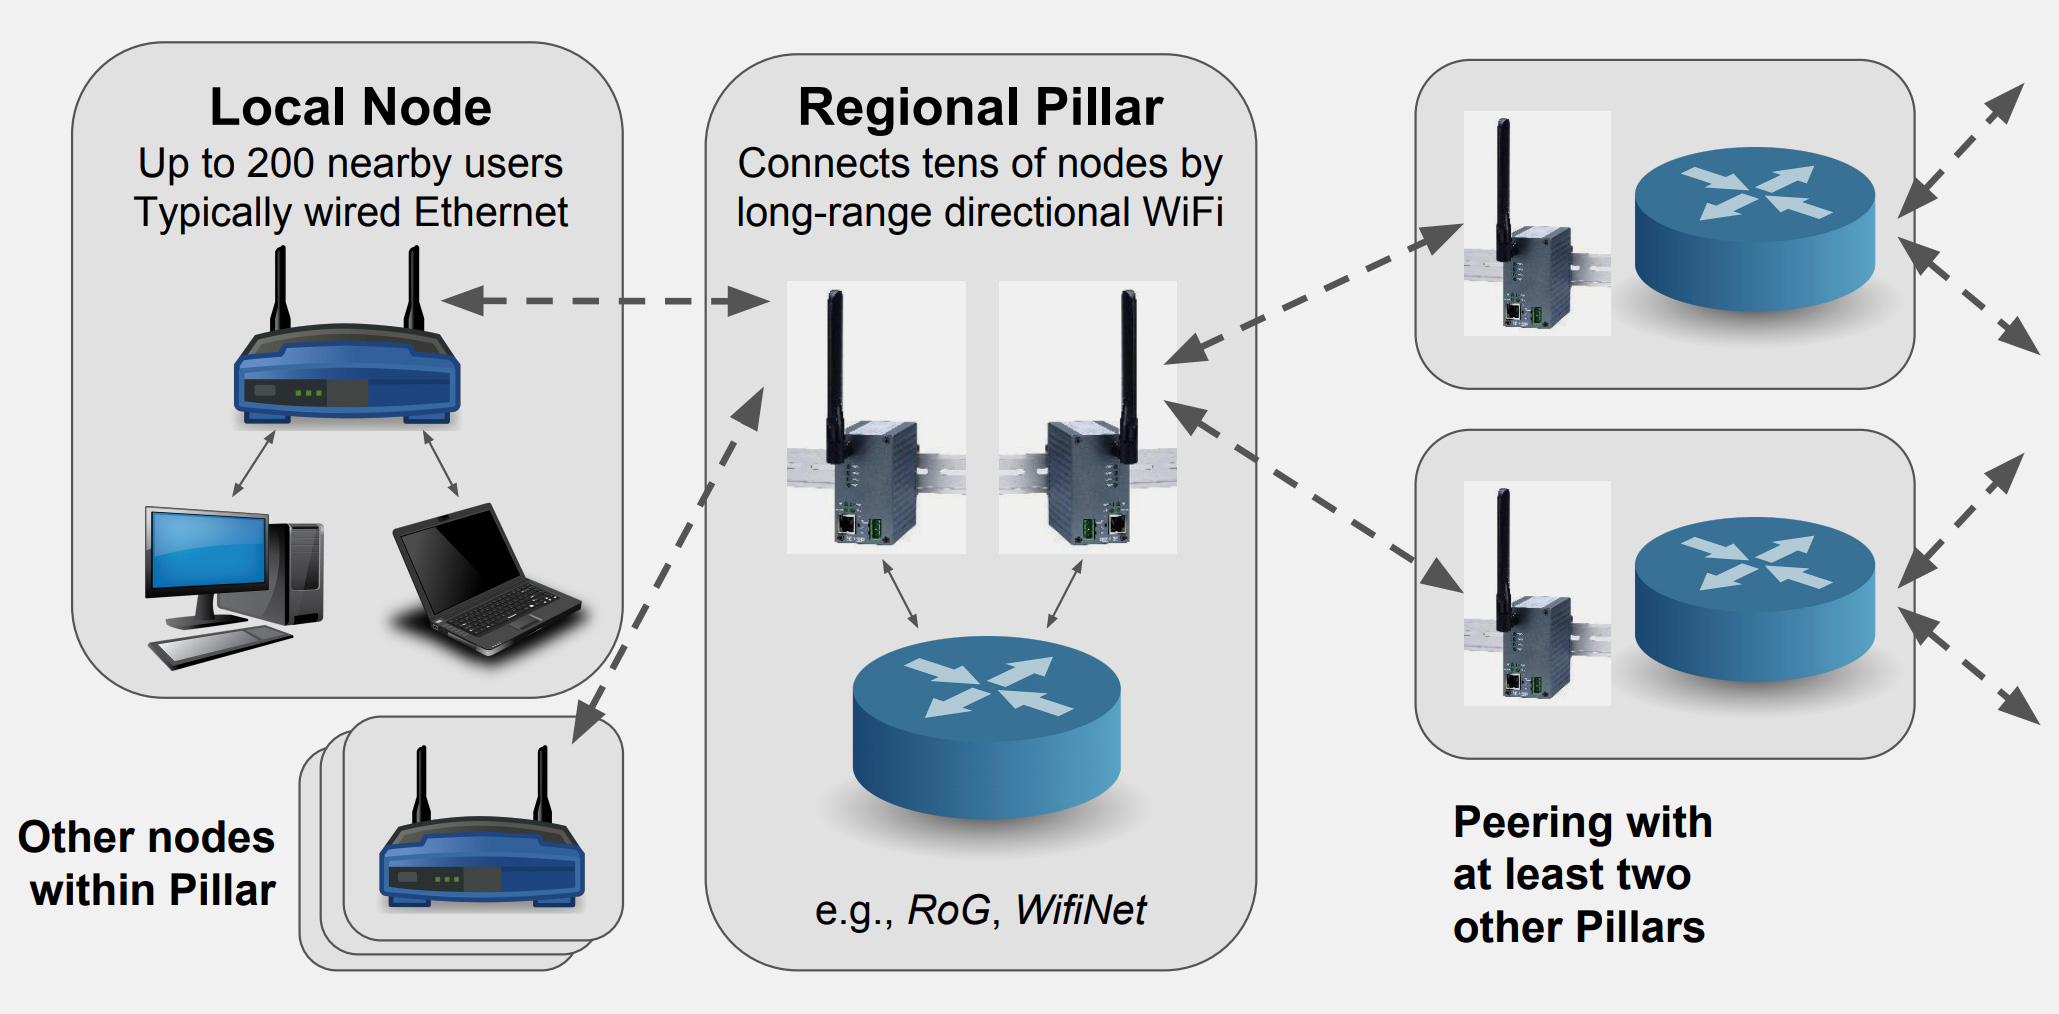
\includegraphics[width=\textwidth]{images/snet_tech.jpg}
	\end{itemize}
	
\end{frame}
		
\begin{frame}
\frametitle{Schaut dann so aus:}
	\begin{itemize}
		\item Günstige Hardware erlaubt es Amateur-Admins viele Knotenpunkte zu maintainen:
			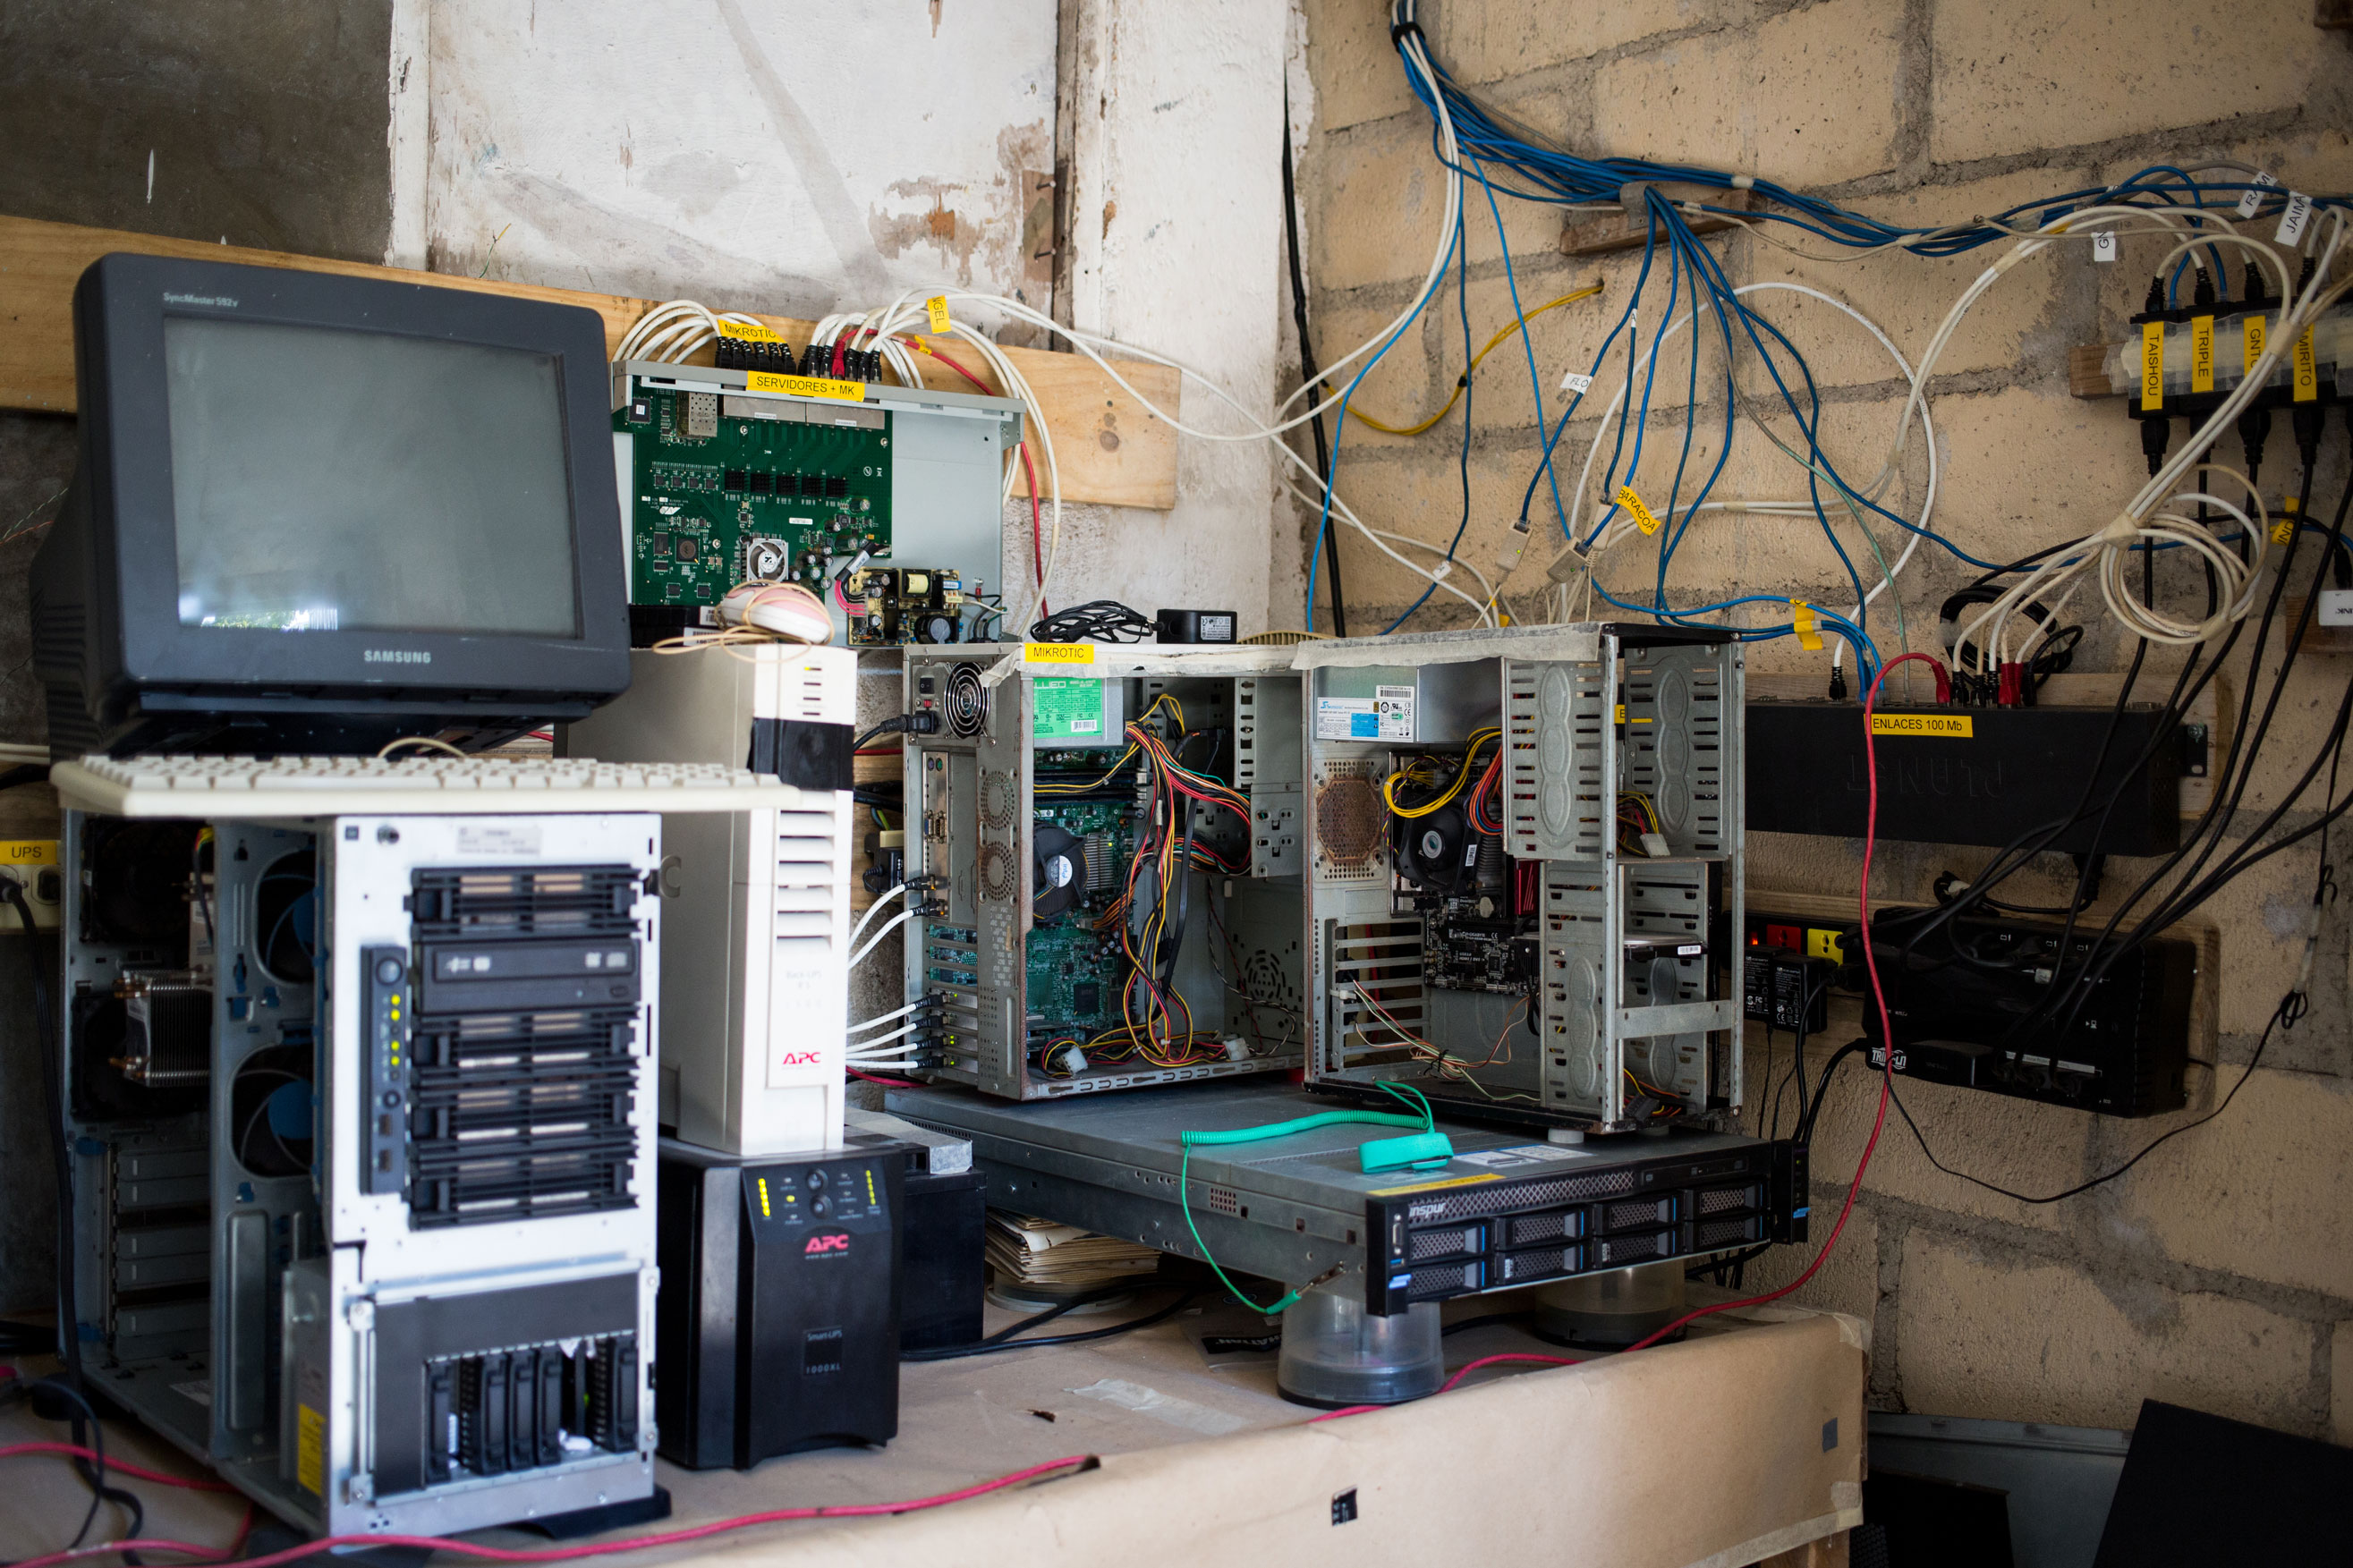
\includegraphics[width=\textwidth]{images/snet_pillar.jpg}
		\item Einziger Nachteil: Veraltete Hardware
	\end{itemize}
\end{frame}

\subsection{Lage in Kuba}

\begin{frame}
\frametitle{}
	\begin{itemize}
		\item Unabhängig von monopolistischen/staatlichen Betreibern - wird von Menschen betrieben, nicht von Institutionen
		\item Schwer zu überwachen, weil dezentral - allerdings befolgen sie selbstgestellte Regeln, wie zB Verbot von Pornographie
	\end{itemize}
\end{frame}
